\documentclass{beamer}
\mode<presentation> {
\usetheme{Boadilla}
}

%%import packages....I didnt use all of these, they're just in my template
\usepackage{graphicx}
\usepackage{booktabs}
\usepackage{standalone}
\usepackage{tikz}
\usepackage{textpos}
\usepackage{modiagram}
\usepackage{physics}
\usepackage{amsmath}
\usepackage[percent]{overpic}
\usepackage{subfig}
\usepackage{xcolor}
\usepackage{subfiles}
\usepackage{hyperref}



\usetikzlibrary{arrows.meta,positioning,decorations.markings,backgrounds}

\tikzset{
    every node/.style={font=\footnotesize},
}

%%citation style parameters

\usepackage[backend=bibtex,%
isbn=false,%
url=false,%
style=authoryear,%
% firstinits=false,
maxbibnames=2,%
]{biblatex}
\bibliography{My Collection.bib}

\renewbibmacro*{cite}{%
  \iffieldundef{shorthand}
    {\ifthenelse{\ifnameundef{labelname}\OR\iffieldundef{labelyear}}
       {\usebibmacro{cite:label}%
        \setunit{\printdelim{nonameyeardelim}}}
       {\printnames{labelname}%
        \setunit{\printdelim{nameyeardelim}}}%
     \usebibmacro{cite:labeldate+extradate}%
     \setunit{\addcomma\space}%
     \usebibmacro{journal}}
    {\usebibmacro{cite:shorthand}}}



%I dont remember why I have this in my template
\usetikzlibrary{decorations.pathreplacing,angles,quotes}

%%UNT color scheme
\colorlet{beamer@blendedblue}{green!40!black}

% Title Information
\title[LIBS]{LIBS of Sputtering Targets}
\author{Brian Squires}
\institute[UNT]
{
University of North Texas \\
\medskip
\textit{Department of Physics}\\
\medskip
\textit{brian.squires@unt.edu}\\
\medskip
\textit{}
}
\date{\today}
% \logo{\vspace{7.25cm}\includegraphics[height=1.5cm]{/Users/briansquires/github/logo1.jpg}}

%Add shaded outline slide before each section
\AtBeginSection[]
{
    \begin{frame}
        \frametitle{Outline}
        \tableofcontents[currentsection]
    \end{frame}
}


\begin{document}
\begin{frame}
    \titlepage    
\end{frame}

\begin{frame}
    \includegraphics[scale=0.5, angle=-90]{/Users/briansquires/Documents/LIBS/IMG_1921.HEIC.pdf}
\end{frame}

\begin{frame}{Average Linewidth = 0.9996nm}
    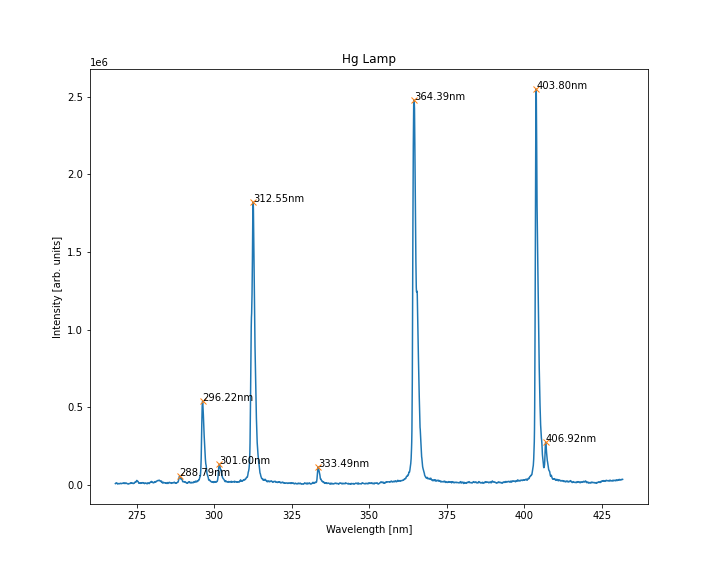
\includegraphics[scale=0.45]{calibrationlamp.png}
\end{frame}

\begin{frame}
    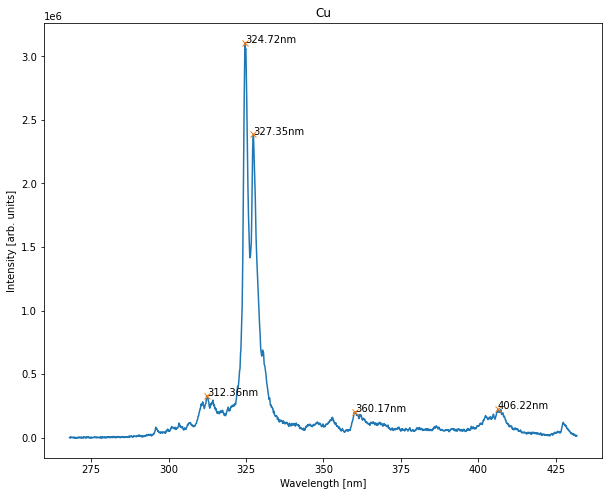
\includegraphics[scale=0.45]{Cu/350nm_10nmslit.png}
\end{frame}

\begin{frame}
    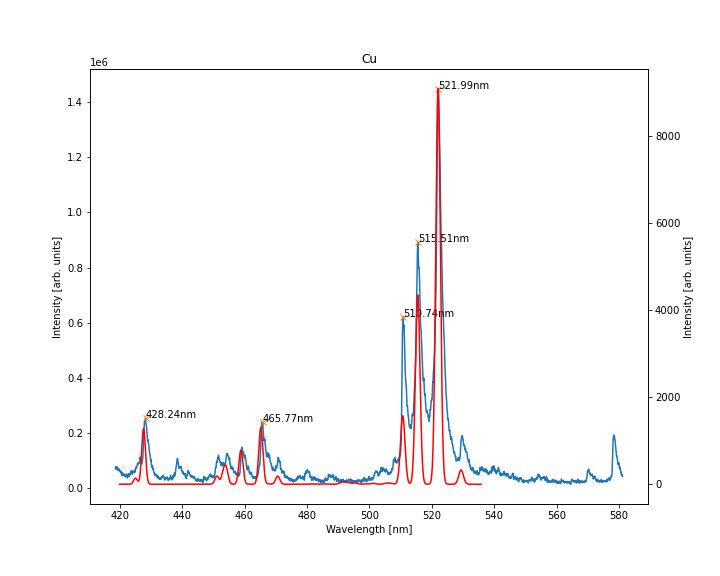
\includegraphics[scale=0.45]{Cu/500nm_10nmslit.png}
\end{frame}

\begin{frame}
    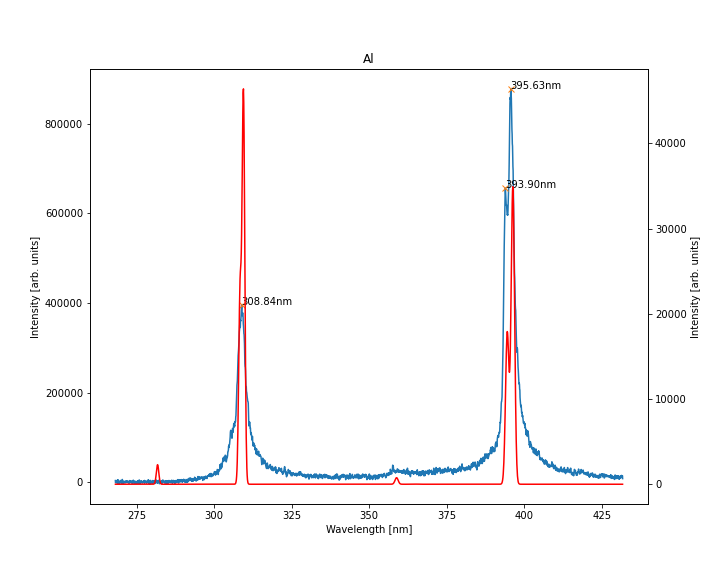
\includegraphics[scale=0.45]{Al/Al_350nm.png}
\end{frame}

\begin{frame}
    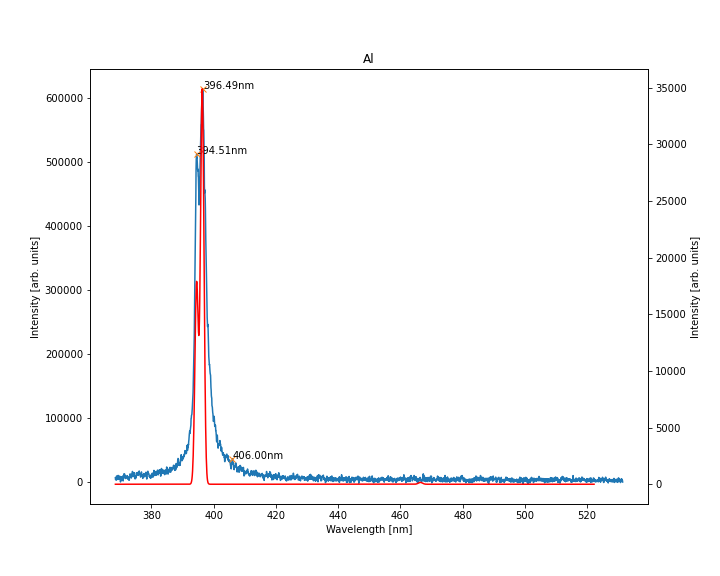
\includegraphics[scale=0.45]{Al/Al_450nm.png}
\end{frame}

\begin{frame}
    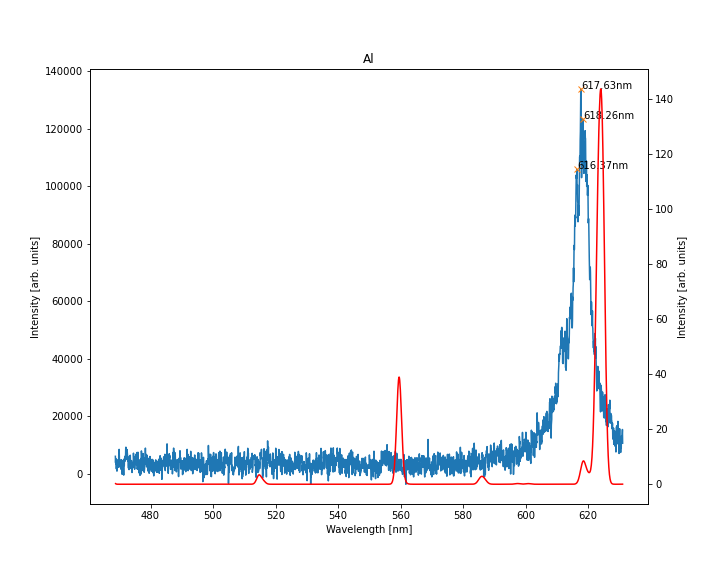
\includegraphics[scale=0.45]{Al/Al_550nm.png}
\end{frame}

\begin{frame}
    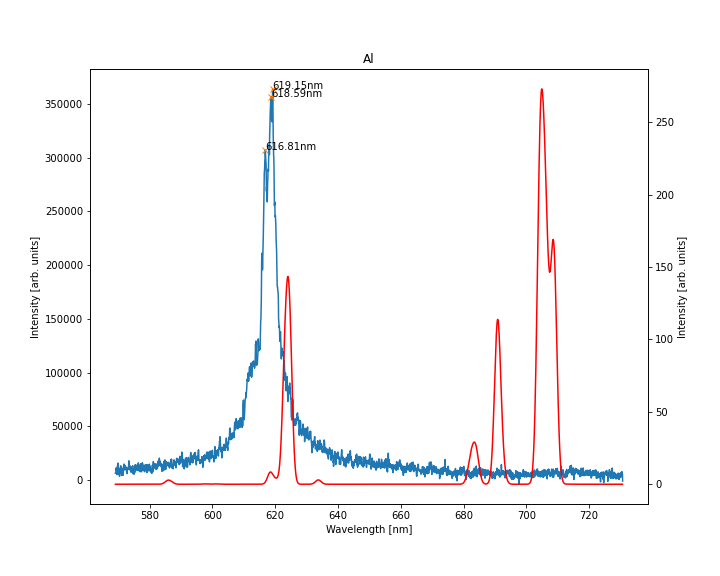
\includegraphics[scale=0.45]{Al/Al_650nm.png}
\end{frame}

\begin{frame}
    \includegraphics[scale=0.45]{Mo/350nm.png}
\end{frame}

\begin{frame}
    \includegraphics[scale=0.45]{Mo/450nm.png}
\end{frame}

\begin{frame}
    \includegraphics[scale=0.45]{Mo/550.png}
\end{frame}

\begin{frame}
    \includegraphics[scale=0.45]{Ni/350nm.png}
\end{frame}

\begin{frame}
    \includegraphics[scale=0.45]{Ni/450nm.png}
\end{frame}

\begin{frame}
    \includegraphics[scale=0.45]{Ni/550.png}
\end{frame}

\begin{frame}
    \includegraphics[scale=0.45]{Ti/350nm.png}
\end{frame}

\begin{frame}
    \includegraphics[scale=0.45]{Ti/450nm.png}
\end{frame}

\begin{frame}
    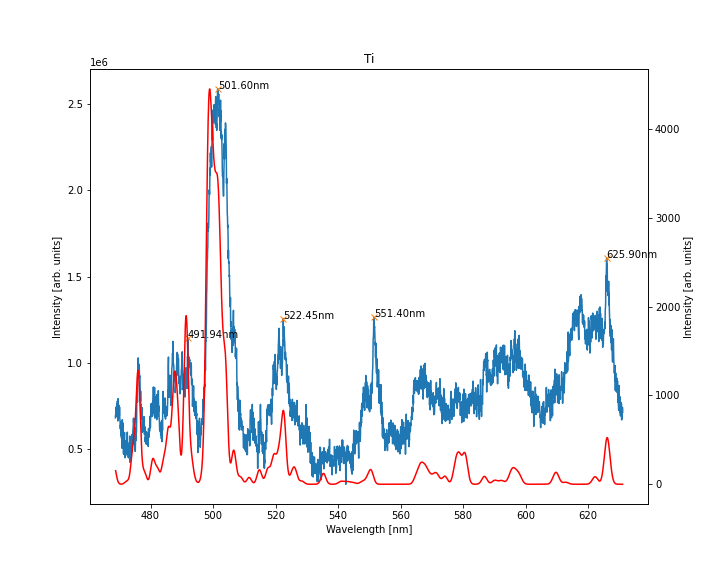
\includegraphics[scale=0.45]{Ti/550nm.png}
\end{frame}

\begin{frame}
    \includegraphics[scale=0.45]{W/350nm.png}
\end{frame}

\begin{frame}
    \includegraphics[scale=0.45]{W/450nm.png}
\end{frame}

\begin{frame}
    \includegraphics[scale=0.45]{W/550.png}
\end{frame}

\begin{frame}
    \includegraphics[scale=0.45]{C/350.png}
\end{frame}

\begin{frame}
    \includegraphics[scale=0.45]{C/450.png}
\end{frame}

\begin{frame}
    \includegraphics[scale=0.45]{C/550.png}
\end{frame}

\begin{frame}
    \includegraphics[scale=0.45]{Fe/350.png}
\end{frame}

\begin{frame}
    \includegraphics[scale=0.45]{Fe/450.png}
\end{frame}

\begin{frame}
    \includegraphics[scale=0.45]{Fe/550.png}
\end{frame}

\begin{frame}{Next Steps}
    \begin{itemize}
        \item Optimize optical collection pathway with new lens
        \begin{itemize}
            \item New lens ordered
            \item Will enhance collection efficiency in UV 
            \item Particularly important for Fe peak at 275nm
        \end{itemize}
        \item Develop machine learning algorithm for concentration analysis 
        \begin{itemize}
            \item see \href{https://www.nature.com/articles/s41598-019-47751-y}{Sun, C., Tian, Y., Gao, L. et al. Machine Learning Allows Calibration Models to Predict Trace Element Concentration in Soils with Generalized LIBS Spectra. Sci Rep 9, 11363 (2019). https://doi.org/10.1038/s41598-019-47751-y}
            \item Confirm with univariate calibration (concentration gradient sample
        \end{itemize}
        \item Perform experiments under blanket of argon
        \begin{itemize}
            \item Mitigate molecular LIBS signal (likely from $O_2$ and metal oxides)
        \end{itemize}
        \item New mirrors to use 520nm excitation
        \begin{itemize}
            \item Should enhance plasma emission by order of magnitude 
            \item problem with fiber coupling 
        \end{itemize}
    \end{itemize}
\end{frame}


\end{document}